%\documentclass[10pt,xcolor=table]{beamer}
\documentclass[notes=only,10pt,xcolor=table]{beamer}
%\documentclass[notes, 10pt,xcolor=table]{beamer}

% Use the preamble setting
% Beamer theme
\usetheme[titleformat=allcaps, progressbar=foot,
          titleformat title=allcaps, titleformat subtitle=allcaps,
          titleformat section=smallcaps, titleformat frame=smallcaps]{metropolis}
% Settings to have progress bar at the top
\useoutertheme[subsection=false]{miniframes}
\useinnertheme{circles}
%% \usefonttheme{structurebold}
\usecolortheme{beaver}

% Some change in font colour
\setbeamercolor{normal text}{fg=black, bg=white}
\setbeamercolor{altered text}{fg=black, bg=white}
\setbeamercolor{example text}{fg=black, bg=white}

% Change in the title color
\definecolor{BostonUniRed}{rgb}{0.8, 0.0, 0.0}
\setbeamercolor{frametitle}{fg=BostonUniRed, bg=BostonUniRed!10}

% Add graphics path
\usepackage{graphicx}
\graphicspath{{img/}{clips/}}

\usepackage{booktabs}
\usepackage[scale=2]{ccicons}

\usepackage{pgfplots}
\usepgfplotslibrary{dateplot}

\usepackage{pifont}

% Define graphics for logo
\titlegraphic{%
  \includegraphics[height=.125\textheight]{BostonUni.png} \hfill
  %\includegraphics[height=.125\textheight]{CEL_Logo.eps}
}
% Setting title page to be centered, and add logos at the bottom
\makeatletter
\setbeamertemplate{title page}{
  \begin{minipage}[b][\paperheight]{\textwidth}
    % Centering titles    
    \centering  % <-- Center here
    \vfill%
    \ifx\inserttitle\@empty\else\usebeamertemplate*{title}\fi
    \ifx\insertsubtitle\@empty\else\usebeamertemplate*{subtitle}\fi
    \usebeamertemplate*{title separator}
    \ifx\beamer@shortauthor\@empty\else\usebeamertemplate*{author}\fi
    \ifx\insertdate\@empty\else\usebeamertemplate*{date}\fi
    \ifx\insertinstitute\@empty\else\usebeamertemplate*{institute}\fi
    \vfill
    % Inserting logo
    \ifx\inserttitlegraphic\@empty\else\inserttitlegraphic\fi    
    \vspace*{10mm}
  \end{minipage}
}
\setbeamertemplate{title}{
%  \raggedright%  % <-- Comment here
  \linespread{1.0}%
  \inserttitle%
  \par%
  \vspace*{0.5em}
}
\setbeamertemplate{subtitle}{
%  \raggedright%  % <-- Comment here
  \insertsubtitle%
  \par%
  \vspace*{0.5em}
}
\makeatother

% Manage frame numbering in beamer's appendixes
\usepackage{appendixnumberbeamer}

% URL
\usepackage{hyperref}

% Citation
%\usepackage[backend=bibtex, style=science]{biblatex}
\usepackage[backend=bibtex]{biblatex}
% Hacky fix to citation
\makeatletter
\def\blx@maxline{77}
\makeatother
% Reduce font size for citation
\setbeamerfont{bibliography item}{size=\footnotesize}
\setbeamerfont{bibliography entry author}{size=\footnotesize}
\setbeamerfont{bibliography entry title}{size=\footnotesize}
\setbeamerfont{bibliography entry location}{size=\footnotesize}
\setbeamerfont{bibliography entry note}{size=\footnotesize}
\renewcommand{\footnotesize}{\tiny}

% Change caption font size
\usepackage[font=scriptsize, labelfont=bf]{caption}
\usepackage{subcaption}

% Box around text
\usepackage{tcolorbox}

% For large table in the timeline
\usepackage{chngpage}


% Title and logo
\title{Operating System Energy-Performance Trade-offs towards System Self Optimization}
\subtitle{Dissertation Proposal}
%\date{\today}
\date{January 24, 2022}
\author{Han Dong}

% Add bibliography file
\bibliography{reference}

\begin{document}
% Make the title
{
% Uncomment the following to dismiss the transparent background crest
\setbeamertemplate{background}{\tikz[remember picture,overlay]\node[opacity=0.04] at (current page.center) {\includegraphics[height=0.8\paperheight,keepaspectratio]{BostonUni_Crest.eps}};}
\maketitle
}

% Setting all titles to be centered
\setbeamertemplate{frametitle}[default][center]

% Table of content
\begin{frame}[plain]{Table of Contents}
  \setbeamertemplate{section in toc}[sections numbered]
  \tableofcontents[hideallsubsections]
\end{frame}

% Section 1
\section{Introduction}

%% TRENDS IN COMPUTING
\begin{frame}
  \frametitle{Trends in computing}
  \only<1>{
  \begin{itemize}
  \item Energy growth in computing.
  \item Hardware increasingly complex, many features packed into it.
  \item Software dedicated to run on a single node within a datacenter.
  \end{itemize}
  }
  \only<2>{
  \begin{itemize}
  \item Energy growth in computing.
  \item Hardware increasingly complex, many features packed into it.
  \item Software dedicated to run on a single node within a datacenter.
  \end{itemize}
  \begin{figure}
    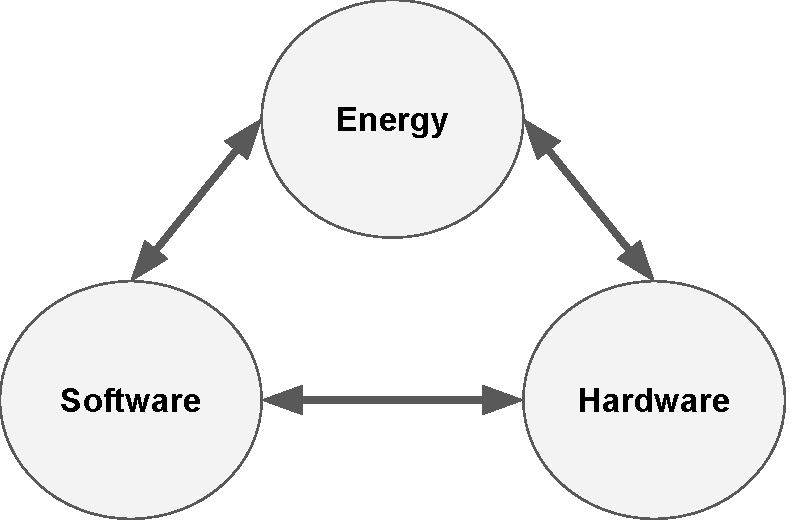
\includegraphics[width=0.65\textwidth]{img/energy-sw-hw-tradeoff.pdf}
    %\caption{Two mantis on a wig.}
  \end{figure}
  }
\end{frame}
%% NOTES
\note{
\begin{itemize}
    \item There are other trends, but I identify these are useful/important to consider with respect to OSes and challenges we face
    \item Relationship between the 3 and questions to be asked in this setup
    \item Point 3 can be exploited to make these things easier
\end{itemize}
}
%%%%%%%%%%%%%%%%%%%%%%%%%%%%

%% ENERGY
\begin{frame}{Energy}
\framesubtitle{Trends in computing}
\begin{columns}
    \begin{column}{.5\textwidth}
        \begin{figure}
            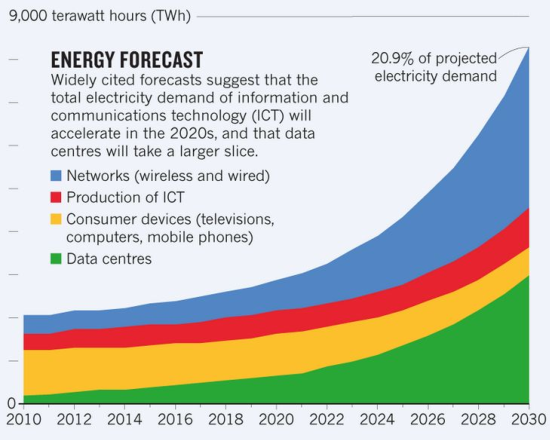
\includegraphics[width=0.9\textwidth]{img/energyuse1.pdf}
            \caption{Nicola Jones, How to stop data centres from gobbling up the world’s electricity, 9/12/2018~\cite{nature1}.}
        \end{figure}
    \end{column}
    \begin{column}{.5\textwidth}
        \begin{figure}
            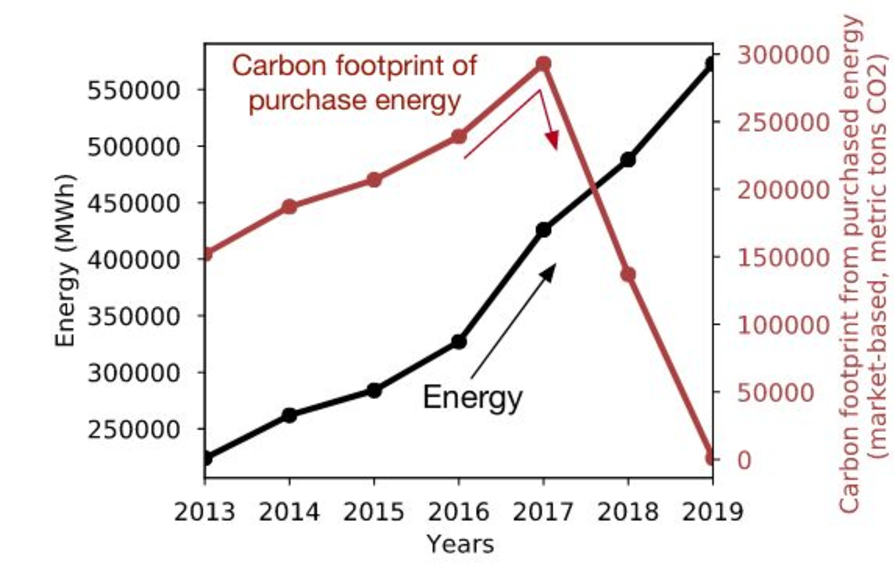
\includegraphics[width=0.9\textwidth]{img/energyuse2.pdf}
            \caption{Udit Gupta et al. Chasing Carbon: The Elusive Environmental Footprint of Computing, 10/28/2020~\cite{gupta2020chasing}.}
        \end{figure}
    \end{column}
    \end{columns}
\end{frame}
\note{
\begin{itemize}
    \item By changing software, exploit more out of existing data center
    \item squeezing more utilization out of existing data center budgets
    \item if energy is free, why does this matter, other impacts -> \textbf{manufacturing & datacenters}, do more work with less energy, more work per computer
\end{itemize}
}
%%%%%%%%%%%%%%%%%%%%%%%%%%%%

%% Hardware Complexity
\begin{frame}{Hardware Complexity}
\framesubtitle{Trends in computing}
    \only<1>{
    \begin{itemize}
        \item Hardware has grown to have more processing logic:
        \begin{itemize}
            \item[\ding{212}] Offload work that used to be done by software.
            \item[\ding{212}] Reflect changing application requirements.
        \end{itemize}
    \end{itemize}
    }
    \only<2>{
    \begin{columns}
      \begin{column}{.4\textwidth}
        \begin{itemize}
        \item Hardware has grown to have more processing logic:
        \begin{itemize}
            \item[\ding{212}] Offload work that used to be done by software.
            \item[\ding{212}] Reflect changing application requirements.
        \end{itemize}
    \end{itemize}
      \end{column}
      \begin{column}{.6\textwidth}
        \begin{figure}
            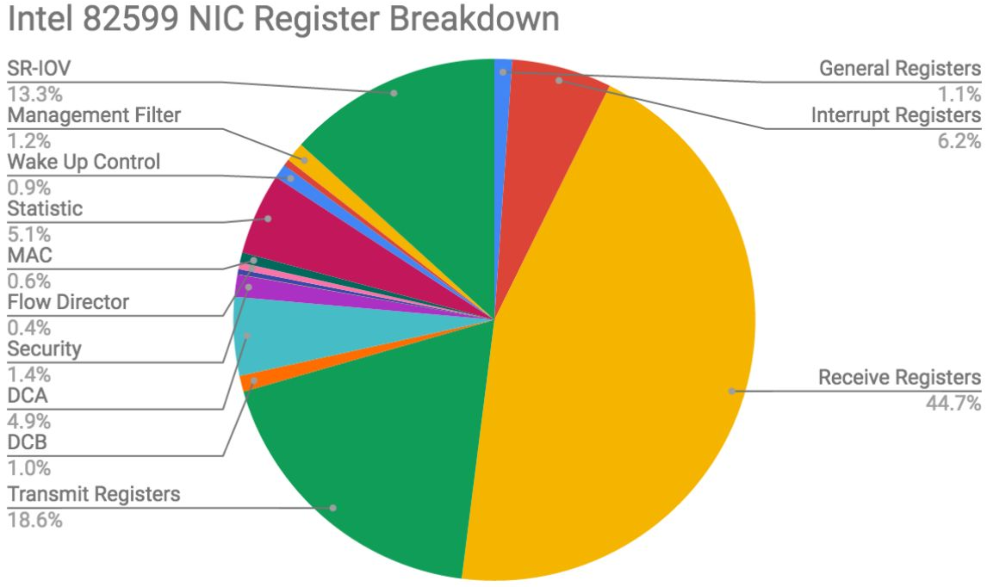
\includegraphics[width=1.0\textwidth]{img/82599_NIC.pdf}
            \caption{Breakdown of table of contents in Intel 82599 10 GbE NIC datasheet~\cite{82599}.}
        \end{figure}
      \end{column}
    \end{columns}
    \note{over 5000 configurable features}
    }
    \only<3>{
    \begin{columns}
      \begin{column}{.4\textwidth}
        \begin{itemize}
        \item Device drivers have grown in complexity to drive these features.
        \item Effectively using these features is dependent on application requirements.
        % \begin{itemize}
        %     \item Software shielded away from needing to manage this sort of complexity.
        % \end{itemize}
    \end{itemize}
      \end{column}
      \begin{column}{.6\textwidth}
        \begin{figure}
            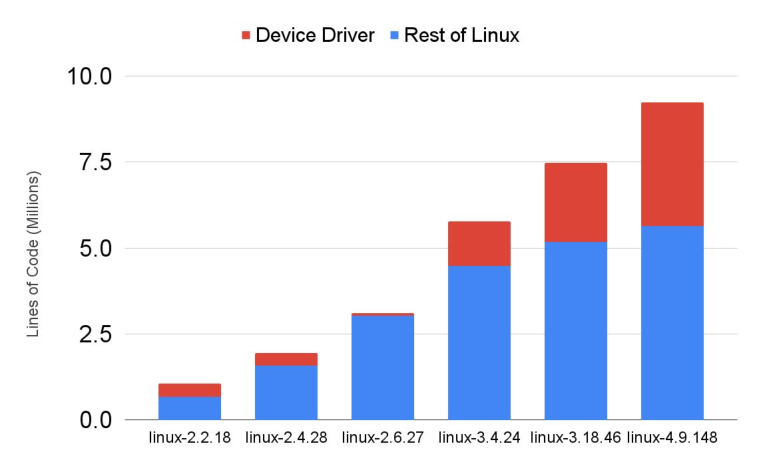
\includegraphics[width=1.0\textwidth]{img/devicedriverloc.pdf}
            \caption{Lines of code measured from Linux kernel in last 10 years using SLOCCount~\cite{sloccount}.}
        \end{figure}
      \end{column}
    \end{columns}
    }
\end{frame}
\note{
\begin{itemize}
    \item NIC does more work in hardware than before
    \item Example features: security, checksum offloading, batching, packet coalescing
    \item Some features offloaded used to be in SW
    \item Software shielded away from needing to manage this sort of complexity.
\end{itemize}
}
%%%%%%%%%%%%%%%%%%%%%%%%%%%%

%% Software Dedication
\begin{frame}{Software Dedication}
\framesubtitle{Trends in computing}
    \only<1>{
    \begin{itemize}
        \item Data center aggregation of all compute with massive amounts of hardware nodes:
        \begin{itemize}
            \item[\ding{212}] Dedication of entire nodes to meet application demand.
        \end{itemize}
    \end{itemize}
    }
    \only<2>{
    \begin{itemize}
        % \item Data center aggregation of all compute with massive amounts of hardware:
        % \begin{itemize}
        %     \item[\ding{212}] Dedication of entire nodes to meet application demand.
        % \end{itemize}
        % \vspace{0.5cm}
        \item Facebook's cluster management system (\textbf{Twine}~\cite{twine}): 
        \begin{itemize}
            \item Elastically scale clusters of many small machines (1 CPU, 64 Gb RAM).
            \item Applications use containers (rather than VMs) for deployment.
            \item Per-node customization's such as NIC settings, kernel versions, sysctl, filesystems, etc.
        \end{itemize}
    \end{itemize}
    }
    \only<3>{
    \begin{itemize}
        \item In academia, renewed interest in building per-application systems~\cite{ix, mica, zygos, shenango, bmcmcd, dynsleep, 10.1145/3132747.3132764, 10.5555/2387880.2387894, segcache, stackmap, seuss, arrakis, rumpkernel, unikernels, aliraza}, such as library OSes, unikernels, kernel-bypass techniques, etc. %, mostly written using modern programming languages such as C/C++, Python, Rust, golang, etc.
        \begin{itemize}
            \item[\ding{212}] Mostly focused on performance, energy efficiency is a largely un-explored.
        \end{itemize}
    \end{itemize}
    }
\end{frame}
\note{
\begin{itemize}
    \item Break down these three trends into a broader question that this thesis poses.
\end{itemize}
}
%%%%%%%%%%%%%%%%%%%%%%%%%%%%

%% Broad thesis motivation
\begin{frame}{Broad Thesis}
\only<1> {
    %\textit{What are the performance and energy trade-offs in exploiting the relationships between software and dedicated hardware?}
    \textit{Significant performance and energy advantages can be obtained by the specializing software and hardware for dedicated use.}
    % Significant performance and energy improvements can be obtained by specializing software for dedicated hardware.
    \note{Break this down into two further sub-observations. 
    \\ If this is true then \\ 
    More compute per-energy, more compute per computer
    \\ More compute can be hosted on existing resources}
    %% dedication that others are tuning for
}
\only<2> {
\begin{columns}
    \begin{column}{.6\textwidth}
        \begin{figure}
            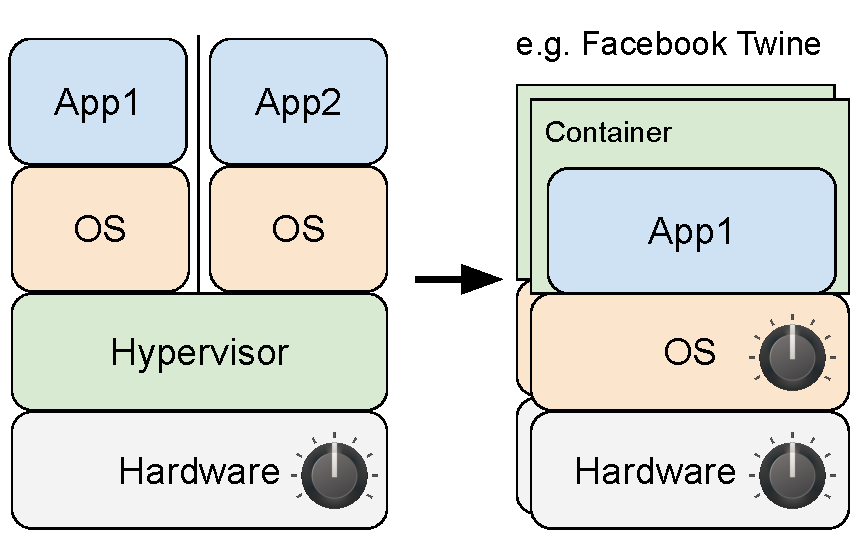
\includegraphics[width=1\textwidth]{img/Hypervisor_to_container.pdf}
        \end{figure}
    \end{column}
    \begin{column}{.4\textwidth}
        \begin{itemize}
            %\item Can OSes better exploit modern hardware features?
            %% Can hardware settings be better exploited to achieve better performance/energy than current use
            %% Can you do this on a general purpose OS?
            %% What is the extent that this can be done?
            %% Evidence that FB has segregated with software settings, how much further can this be exploited?
            %% Add arrows to delineate demand curves
            \item Fine-grained segregation of work permits advantages from specializing hardware settings in an OS and application specific manner.
        \end{itemize}
    \end{column}
\end{columns}
}
\note{What is the extent that this can be done for energy? How much further can this be exploited?}
\only<3> {
\begin{columns}
    \begin{column}{.6\textwidth}
        \begin{figure}
            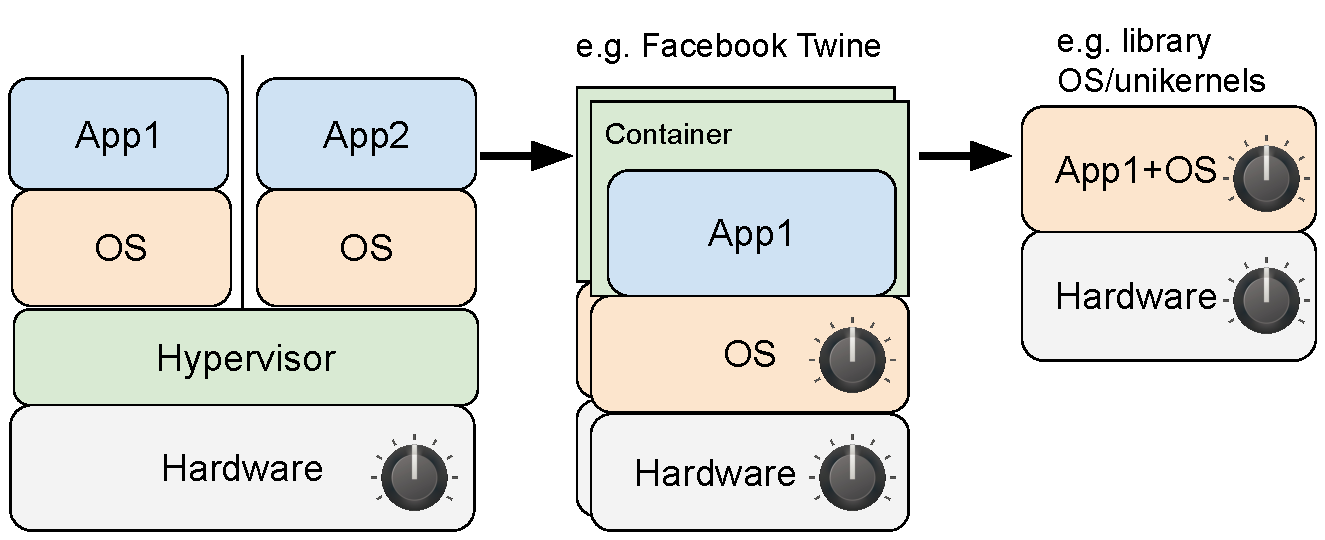
\includegraphics[width=1\textwidth]{img/Hypervisor_to_libos.pdf}
        \end{figure}
    \end{column}
    \begin{column}{.4\textwidth}
        \begin{itemize}
            \item Run application specific OSes on dedicated hardware.
            \item Specialized OSes magnify benefits from specializing hardware settings in an application specific manner.
            % \begin{itemize}
            %     \item[\ding{212}] Energy efficiency of these specialized OSes?
            %     \item[\ding{212}] Benefits of using specialized OSes to exploit modern hardware features?
            % \end{itemize}
        \end{itemize}
        %% aSpecialized OS designs support single app maginify and expand advantages for particular node
        %% Add question to bottom
    \end{column}
\end{columns}
}
\end{frame}
%%%%%%%%%%%%%%%%%%%%%%%%%%%%

%% Thesis Contributions
\section{Thesis Contributions}
\note{My thesis contribution is to go explore this with existing hardware, scope it to a few concrete settings (constrained setting) and why they interact with hardware
}
\begin{frame}{Thesis Contributions Overview}
\only<1>{
    \begin{enumerate}
        \item Identified two hardware features that are easily configured to impact network application performance and energy.
    \end{enumerate}
}
\only<2>{
    \begin{enumerate}
        \item Identified two hardware features that are easily configured to impact network application performance and energy.
        \item Selected and ported four diverse network applications to run on two different OSes.
    \end{enumerate}
}
\only<3>{
    \begin{enumerate}
        \item Identified two hardware features that are easily configured to impact network application performance and energy.
        \item Selected and ported four diverse network applications to run on two different OSes.
        \item Build a novel methodology and test bed to enable this hardware exploration in the different OSes.
    \end{enumerate}
}
\only<4>{
    \begin{enumerate}
        \item Identified two hardware features that are easily configured to impact network application performance and energy.
        \item Selected and ported four diverse network applications to run on two different OSes.
        \item Build a novel methodology and test bed to enable this hardware exploration in the different OSes.
        \item Data analysis of results to gain better insight into software and hardware impacts.
    \end{enumerate}
}
\end{frame}
%%%%%%%%%%%%%%%%%%%%%%%%%%%%

%% Methodology
\section{Methodology}

%% overview
\begin{frame}
\only<1>{
\frametitle{Core Ideas}
There are three aspects of a system that impact the performance and energy of application packet processing: 
\begin{enumerate}
    \item Efficiency of OS networking paths.
    \item Batching of incoming packets.
    \item Frequency of the processor.
\end{enumerate}
\begin{figure}
    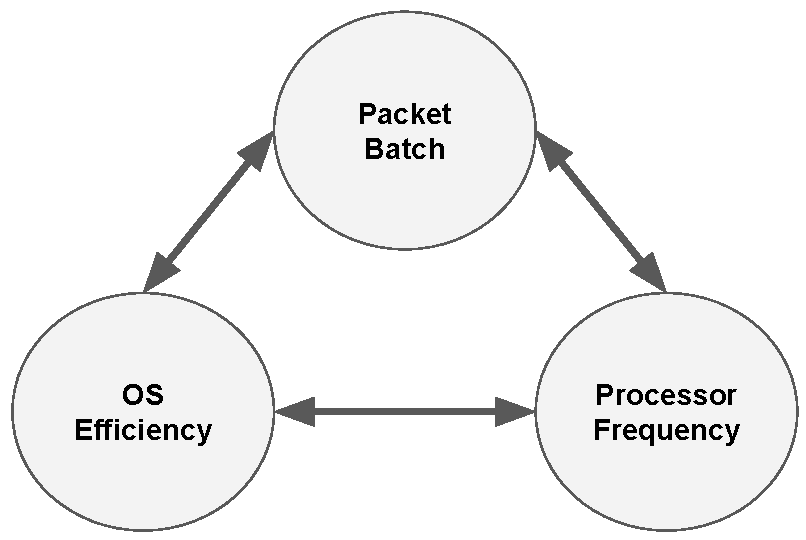
\includegraphics[width=0.6\textwidth]{img/os_batch_proc.pdf}
\end{figure}
\note{
\begin{itemize}
    \item OS Efficiency - library OS, unikernels, kernel bypass techniques
    \item Packet Batch - Frequently done by software, coalesce packets, throttle
    \item Processor Frequency - speed of processor impacts instruction execution, use less energy with slow processor
\end{itemize}
}
}
\only<2>{
\frametitle{OS Efficiency}
\framesubtitle{Core Ideas}
\begin{figure}
    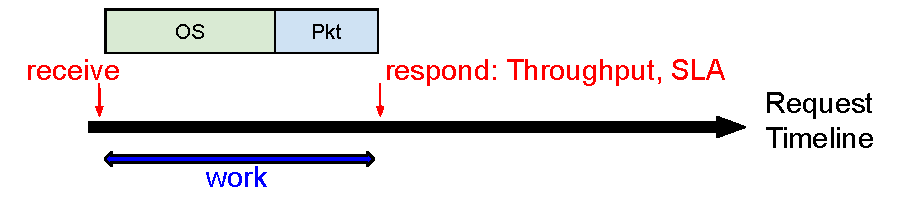
\includegraphics[width=1\textwidth]{img/timeline_os_efficiency1.pdf}
\end{figure}
}
\only<3>{
\frametitle{OS Efficiency}
\framesubtitle{Core Ideas}
\begin{figure}
    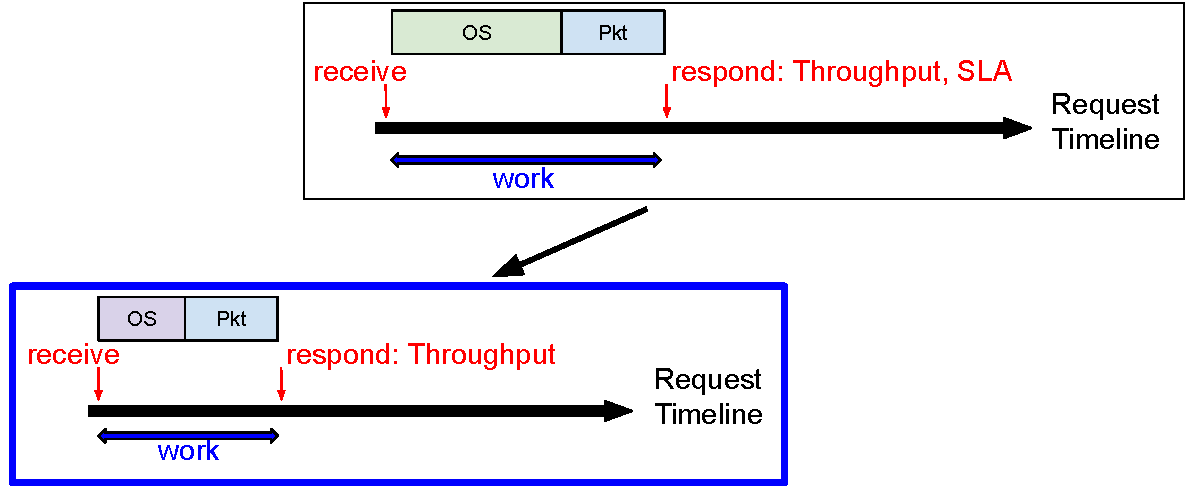
\includegraphics[width=1\textwidth]{img/timeline_os_efficiency2.pdf}
\end{figure}
}
\only<4>{
\frametitle{OS Efficiency}
\framesubtitle{Core Ideas}
\begin{figure}
    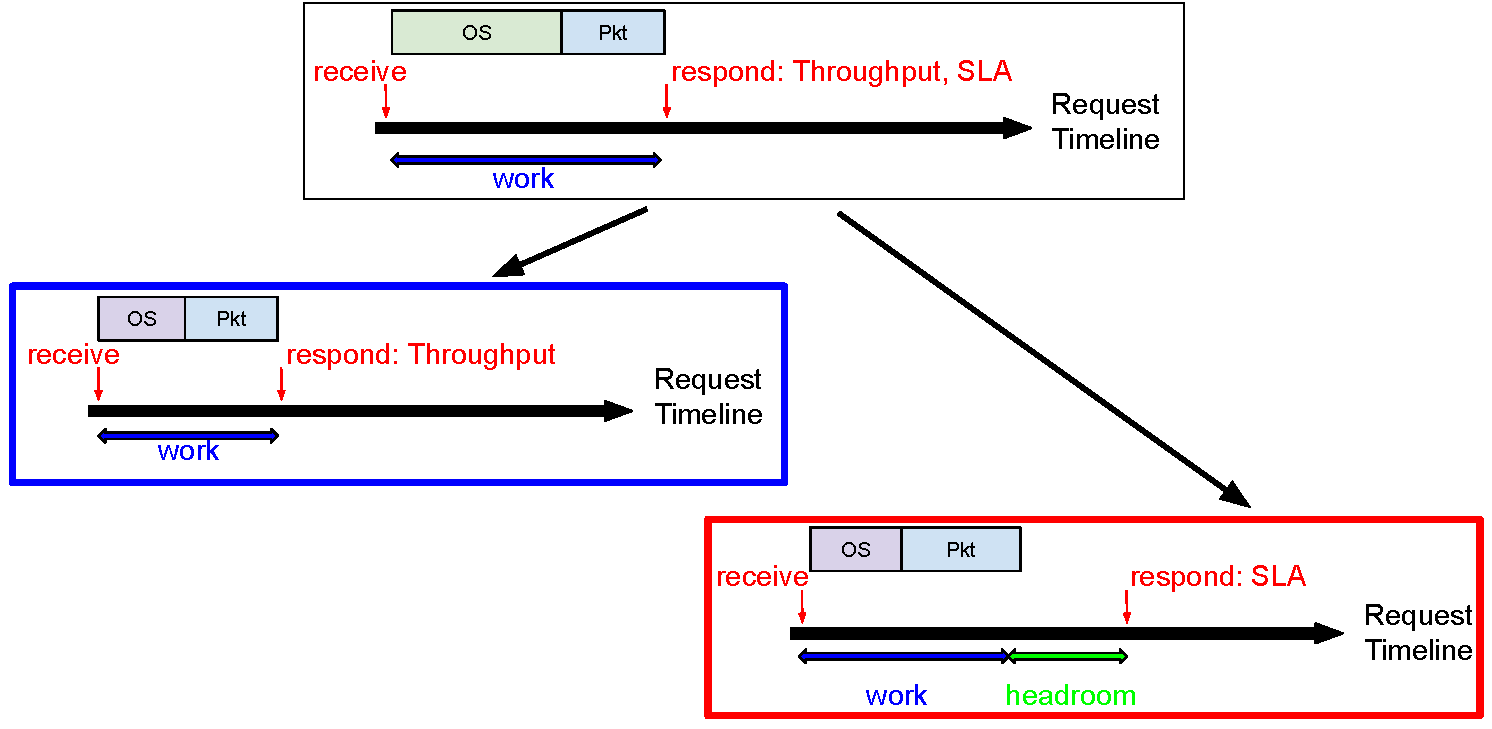
\includegraphics[width=1\textwidth]{img/timeline_os_efficiency3.pdf}
\end{figure}
}
\only<5>{
\frametitle{Packet Batch}
\framesubtitle{Core Ideas}
\begin{figure}
    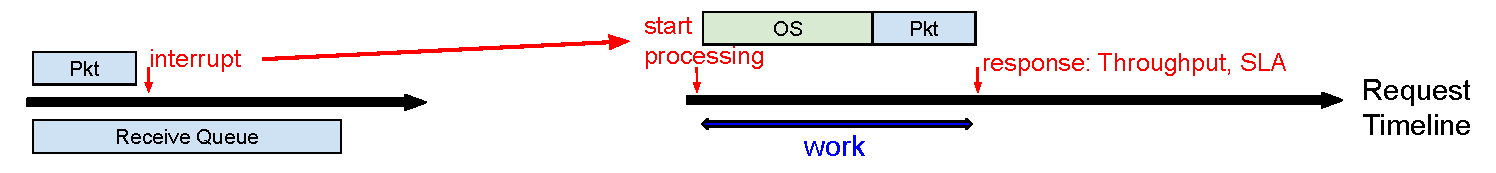
\includegraphics[width=1\textwidth]{img/timeline_batch1.pdf}
\end{figure}
}
\only<6>{
\frametitle{Packet Batch}
\framesubtitle{Core Ideas}
\begin{figure}
    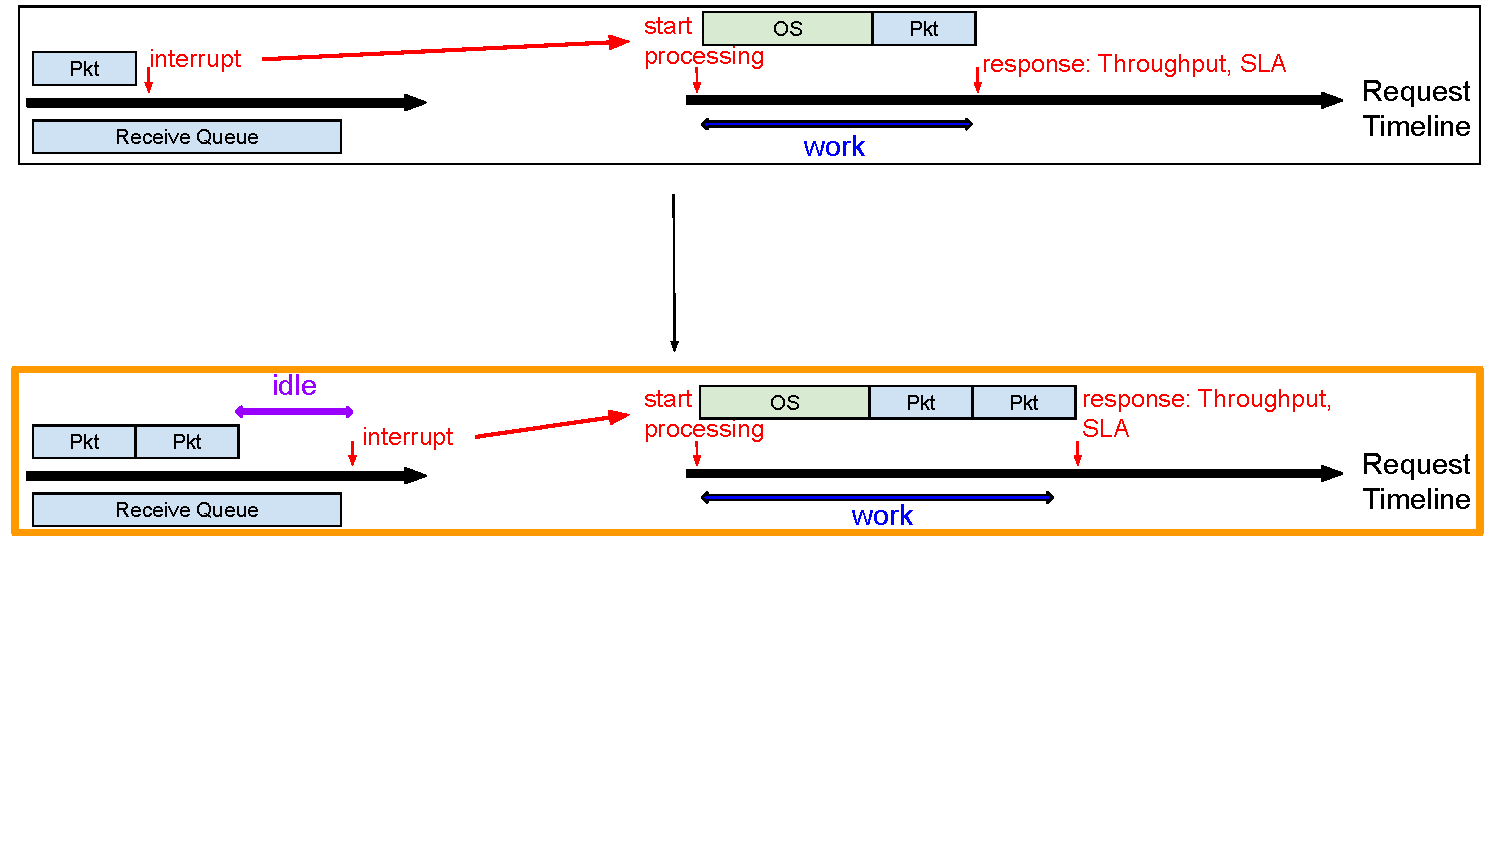
\includegraphics[width=1\textwidth]{img/timeline_batch2.pdf}
\end{figure}
}
\only<7>{
\frametitle{Processor Frequency}
\framesubtitle{Core Ideas}
\begin{figure}
    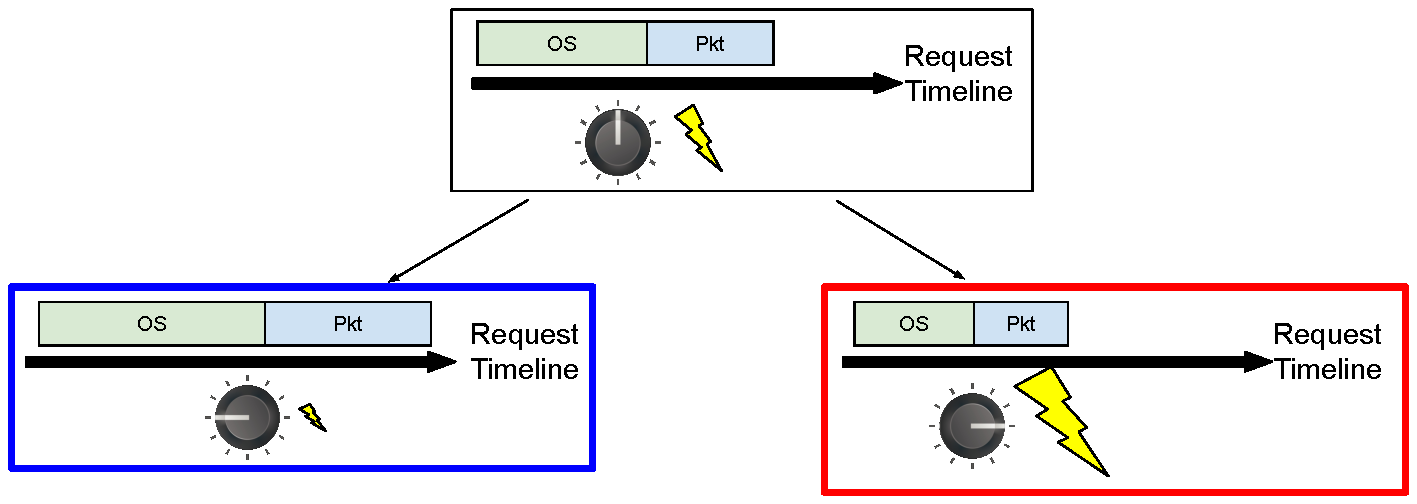
\includegraphics[width=1\textwidth]{img/timeline_dvfs1.pdf}
\end{figure}
}
\end{frame}
\note{
\begin{itemize}
    \item 1+2 direct impact on 3
    \item Per packet optimal work that gets best amortization while not violating performance goals
    \item describe two hardware setting explored in this thesis
    \item finding the ideal batch is an attribute of the software
\end{itemize}
}
%%%%%%%%%%%%%%%%%%%%%%%%%%%%

%% EbbRT
\begin{frame}{Specialized OS}
\framesubtitle{Mechanism}
EbbRT~\cite{ebbrt}, a framework for building per-application library OSes, is used as a mechanism to explore how specialized systems are able to exploit these hardware settings:
\begin{itemize}
    \item Event-driven system
    \item Run-to-completion off a single interrupt
    \item Application and kernel code run in the same domain
    \item Zero-copy of all device buffers to application
    \item 20K lines of code
\end{itemize}
\end{frame}
%%%%%%%%%%%%%%%%%%%%%%%%%%%%

%% ITR
\begin{frame}{NIC Interrupt Delay (ITR)}
\framesubtitle{Mechanism}
\only<1> {
\begin{columns}
    \begin{column}{.5\textwidth}
        \begin{figure}
            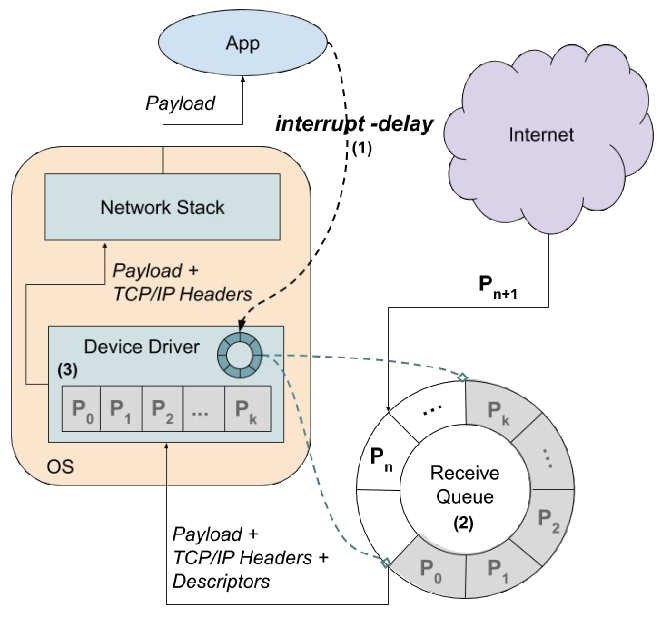
\includegraphics[width=1\textwidth]{img/itr_fig.pdf}
        \end{figure}
    \end{column}
    \begin{column}{.5\textwidth}
        \begin{enumerate}
        %{As interrupt delay (1) is increased, the receive queue (2) buffers more incoming packets as the NIC cannot fire new interrupts until the delay value has been reached. Once the interrupt is fired, Linux's NAPI polling mechanism kicks in and starts pulling in new packets (3) to be processed until it either reaches its current work budget (calculated using existing jiffies) or until there is no more data to be processed.
            \item set ITR to some value
            \item receive queue buffers incoming packets until ITR value has been reached
            \item NIC fires interrupt and packets gets processed by software
            \item NIC delay as a control to induce packet batched processing
        \end{enumerate}
    \end{column}
\end{columns}
}
\only<2>{
\begin{itemize}
    \item Control packet batching behavior.
    \item Hardware values: 0 us - 1024 us, units of 2 us
    \item Batching benefits versus latency trade-offs~\cite{mootaz}
    \begin{itemize}
        \item[\ding{212}] Interacts with energy savings from idle states.
        %\item[\ding{212}] Can also be found on modern RDMA devices~\cite{mellanoxsinterrupt}.
    \end{itemize}
\end{itemize}
\begin{figure}
    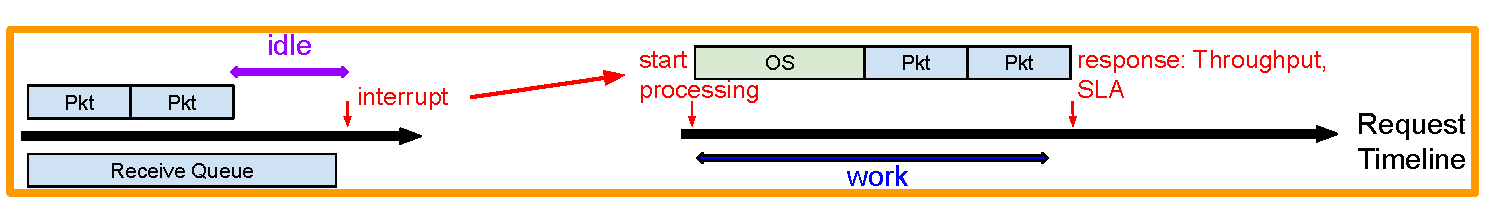
\includegraphics[width=1\textwidth]{img/timeline_batch_individual.pdf}
\end{figure}
}
\end{frame}
\note{this is first work to use ITR has a way to control batching, which induces packet amortization. The NIC as a mechanism for batching}
%%%%%%%%%%%%%%%%%%%%%%%%%%%%

%% DVFS
\begin{frame}{Dynamic Voltage Frequency Scaling (DVFS)}
\framesubtitle{Mechanism}
Control processor frequency and energy, commonly defined as:
\[ P = C f V^2 + P_{static} \]

Hardware values: 1.3 GHz - 2.9 GHz, units of 0.1 GHz.
Trades off instruction execution speed with reduction in energy use. Interacts with both ITR and efficiency of the system.
\end{frame}
\note{
\begin{itemize}
    \item P Is the dynamic power
    \item C Is the switching capacitance (Capacitance is the ability of a component or circuit to collect and store energy in the form of an electrical charge) of the logic circuit 
    \item V Is the operational voltage.
    \item f Is the operational frequency
    \item linear relationship between power consumption and operational frequency.
    \item ITR can batch a lot of work, but do you want to do that if DVFS is slow
    \item  Given a efficient system (i.e. less code to run, more optimized paths), can push DVFS lower to lower energy without sacrificing performance
\end{itemize}
}
%%%%%%%%%%%%%%%%%%%%%%%%%%%%

%% Applications
\begin{frame}{Application Set}
\begin{columns}
    \begin{column}{.5\textwidth}
        \begin{figure}
            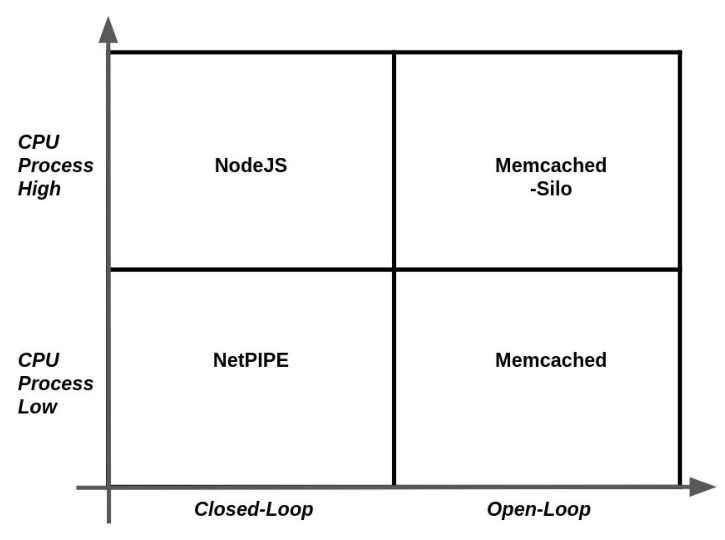
\includegraphics[width=1\textwidth]{img/workload_fig.pdf}
        \end{figure}
    \end{column}
    \begin{column}{.5\textwidth}
        \begin{itemize}
            \item \textbf{NetPIPE}: Ping-pong same sized messages.
            \item \textbf{NodeJS}: HTTP Web Server serving web pages running on NodeJS runtime.
            \item \textbf{Memcached}: Run a real world workload from Facebook ETC~\cite{workloadanalysisfacebook}, SLA: 99\% tail latency $<$ 500 us.
            \item \textbf{Memcached-silo}: Runs a set of TPC-C transactions on an in-memory database (Silo~\cite{silo}) per Memcached request, SLA: 99\% tail latency $<$ 500 us.
        \end{itemize}
    \end{column}
\end{columns}
\end{frame}
\note{changes OS-APP component, changes deadline, arrival rate setting affect gaps on timeline.}
%%%%%%%%%%%%%%%%%%%%%%%%%%%%

%% Test bed
\begin{frame}
\only<1>{
\frametitle{Data Collection Test Bed}
\begin{figure}
    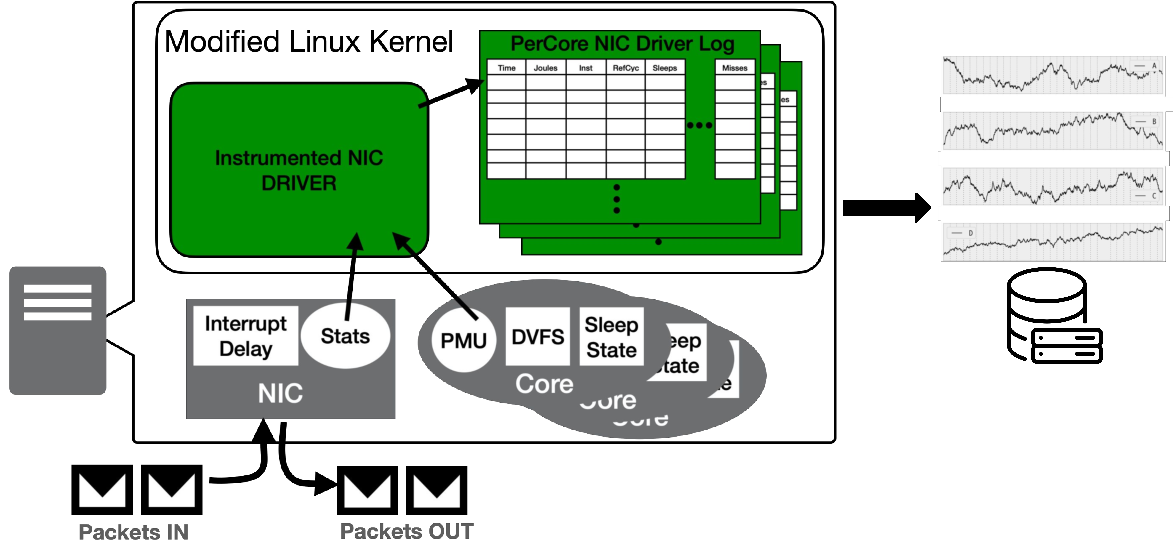
\includegraphics[width=1\textwidth]{img/setup2.pdf}
\end{figure}
RAPL~\cite{intel_rapl} registers to read per-CPU package energy at 1 millisecond rate.

\note{
\begin{itemize}
    \item Enable static ITR+DVFS setting
    \item Instrument logging of hardware performance monitoring counters and software (i.e. instructions, cycles, bytes, descriptors, energy, etc) into interrupt path of device driver
    \item Build a TFTP server based infrastructure to broadcast Linux appliance
    \item Output includes performance, energy, log data with all statistics
    \item booting
    \item controlling noise
    \item moving data on-off
\end{itemize}
}
}
\only<2>{
\frametitle{Data Collection}
\begin{figure}
    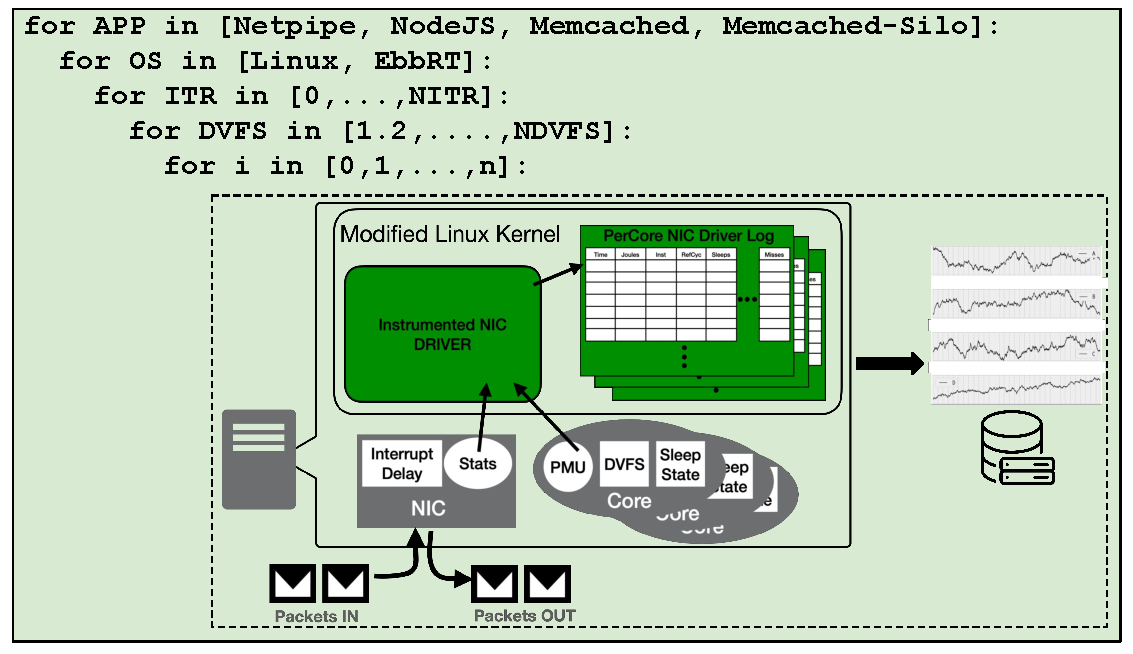
\includegraphics[width=1\textwidth]{img/data_collection.pdf}
\end{figure}
}
% %\noindent\makebox[\linewidth]{\rule{\paperwidth}{0.4pt}}
% \begin{figure}
%     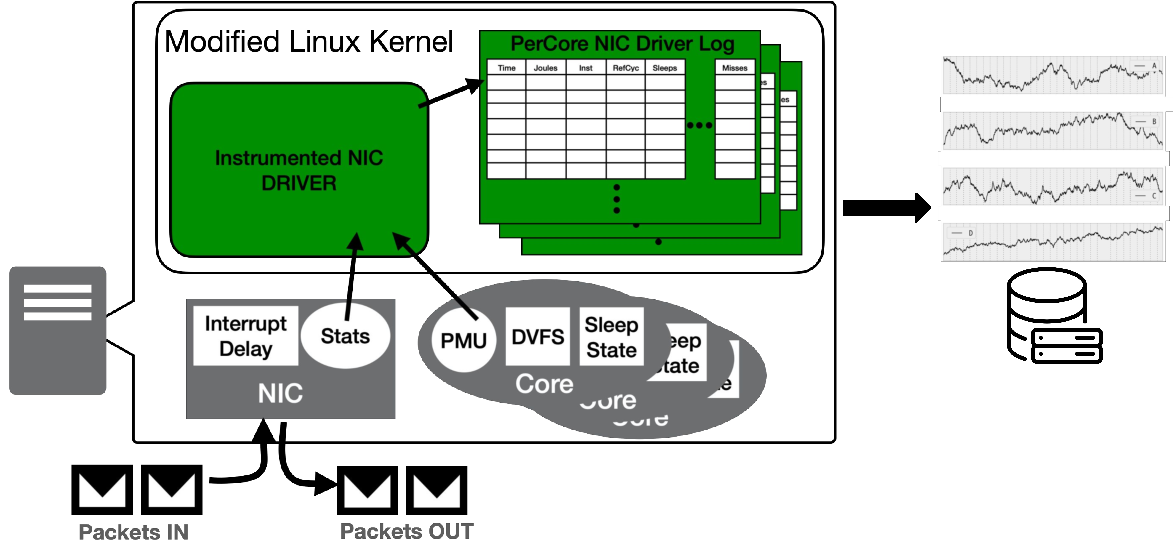
\includegraphics[width=0.8\textwidth]{img/setup2.pdf}
% \end{figure}
\end{frame}
%% Loop that statically sets ITR, DVFS and rerun APPs
%%%%%%%%%%%%%%%%%%%%%%%%%%%%

%% Visualization
\begin{frame}{Visualization Tool}
\begin{figure}
    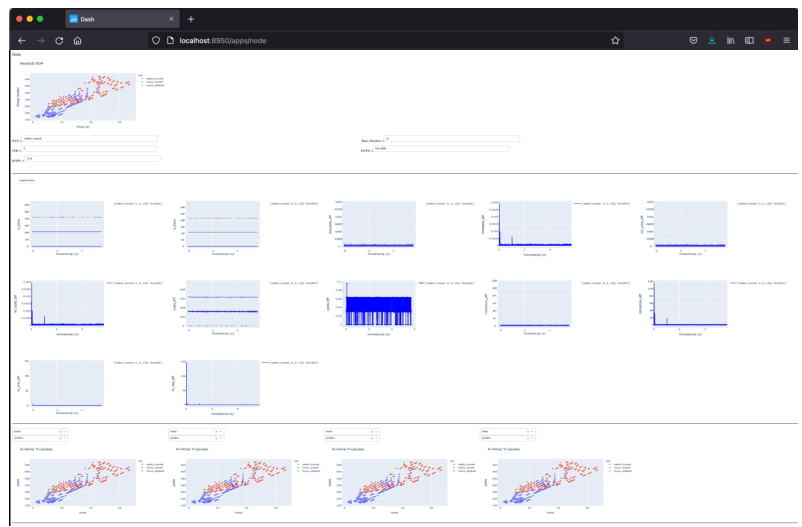
\includegraphics[width=1\textwidth]{img/python_dash_fig.pdf}
\end{figure}
\end{frame}
%%%%%%%%%%%%%%%%%%%%%%%%%%%%

% Results
\section{Experimental Study}

%% data gather
\begin{frame}{Data Gathering Statistics}
\begin{columns}
    \begin{column}{.5\textwidth}
        \begin{figure}
            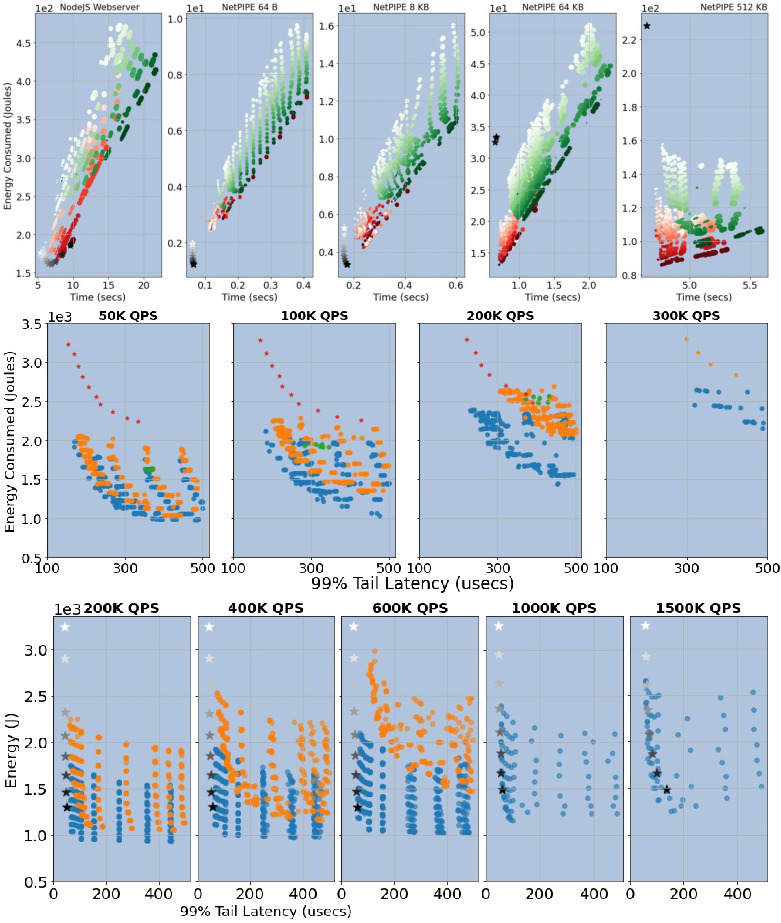
\includegraphics[width=1\textwidth]{img/data_collage.pdf}
        \end{figure}
    \end{column}
    \begin{column}{.5\textwidth}
        \begin{itemize}
            \item Up to 340 unique combinations of ITR, DVFS values.
            \item Repeated up to 10 times for experimental stability.
            \item Total log data contains over 5 TB of data.
        \end{itemize}
    \end{column}
\end{columns}    
\end{frame}
%%%%%%%%%%%%%%%%%%%%%%%%%%%%

%%
\begin{frame}{A use case for the data}
\begin{columns}
    \begin{column}{.5\textwidth}
        \begin{figure}
            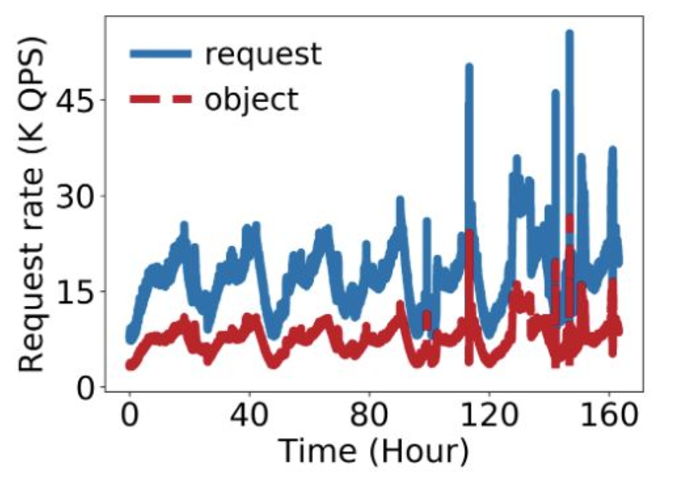
\includegraphics[width=1\textwidth]{img/twitter_mcd.pdf}
            \caption{Twitter key-value store workload trace~\cite{twittermcd}.}
        \end{figure}
    \end{column}
    \begin{column}{.5\textwidth}
        \begin{figure}
            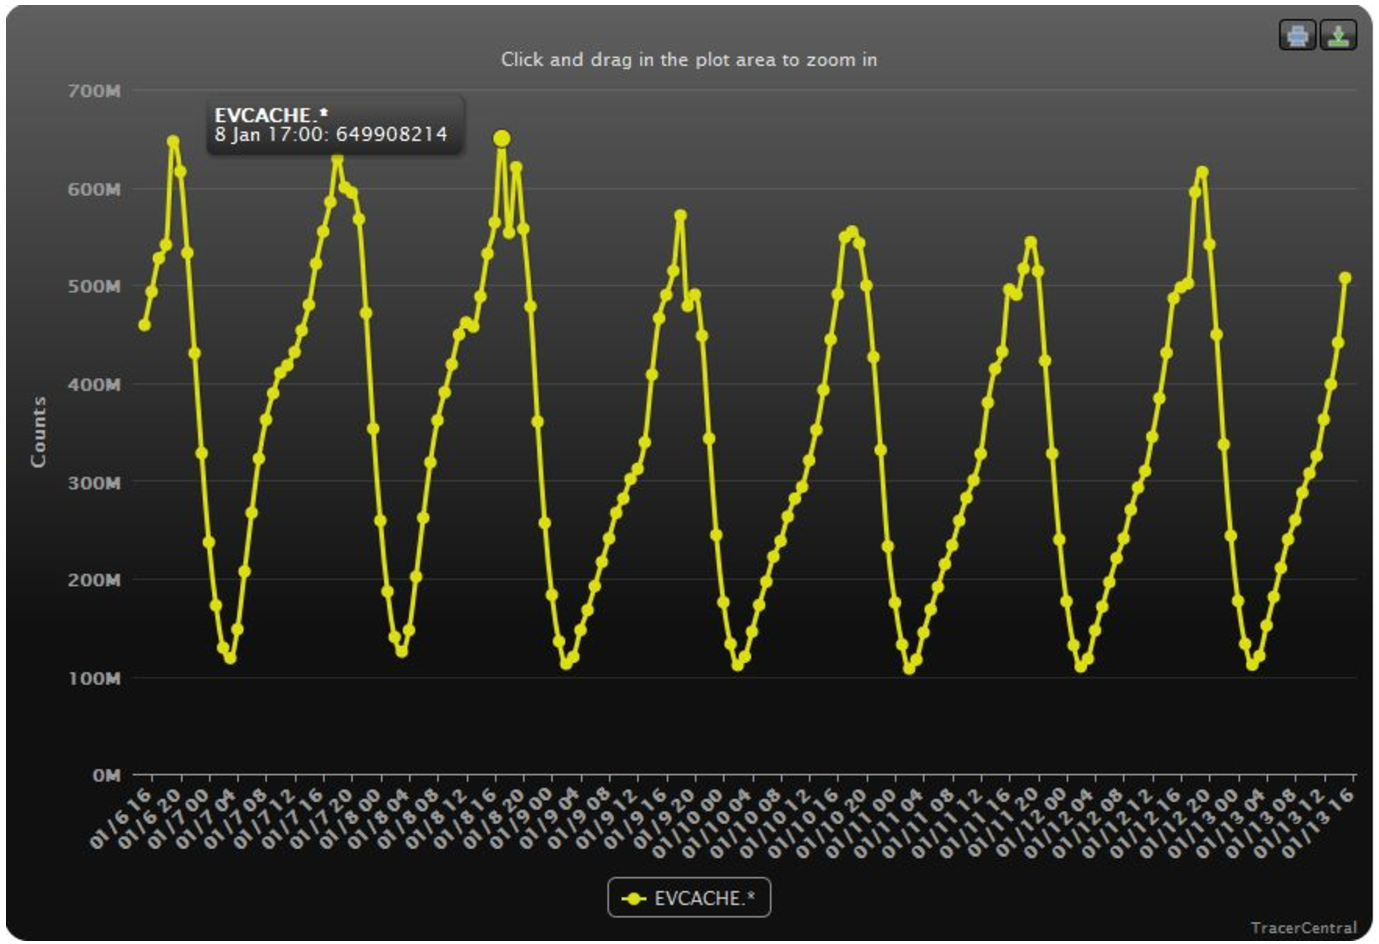
\includegraphics[width=1\textwidth]{img/netflix_mcd.pdf}
            \caption{Netflix key-value store workload trace~\cite{netflixmcd}.}
        \end{figure}
    \end{column}
\end{columns}    
\end{frame}
\note{Exploit mean demand curve that remain relatively stable over multiple hours.}
%%%%%%%%%%%%%%%%%%%%%%%%%%%%

%% findings 1
\begin{frame}{Example Results (under submission to USENIX ATC)}
\begin{columns}
    \begin{column}{.6\textwidth}
        \begin{figure}
            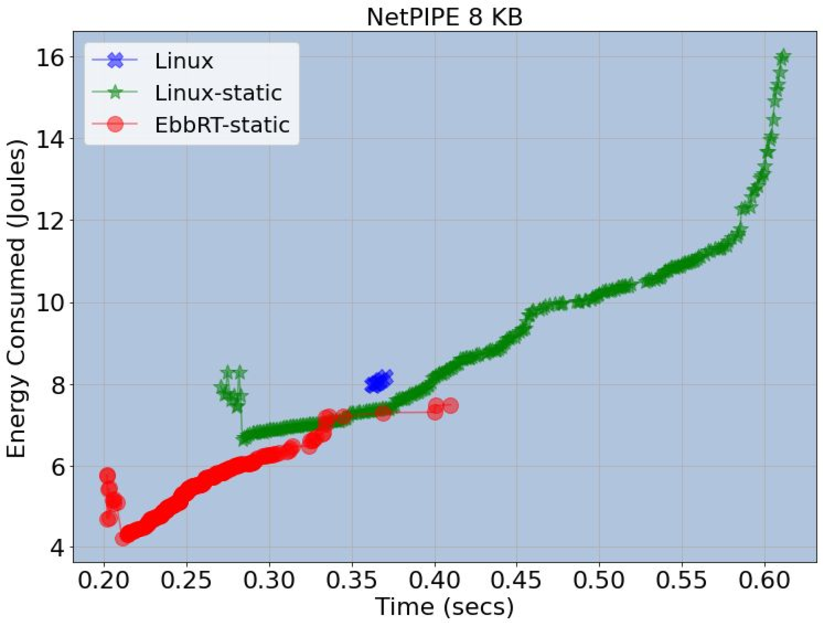
\includegraphics[width=1\textwidth]{img/netpipe8KB.pdf}
        \end{figure}
    \end{column}
    \begin{column}{.4\textwidth}
        \begin{itemize}
            \item 'V' shape
            \item Pareto-optimal curve~\cite{pareto}
            \item ITR scaling with message size
        \end{itemize}
    \end{column}
\end{columns}  
\end{frame}
\note{
\begin{itemize}
    \item  \small The lowest point in this 'V' shape represents a setting that used the lowest energy while being competitive in performance; the vertical points above represent other configurations that sacrifice energy for better performance. We also note that Linux with dynamic settings always lies to the right of the 'V' curve, indicating the value of doing such a static search
    \item \small ITR value is used to effectively determine how much payload the software should process in a fixed quantum. With much larger message sizes, portions of its payload being transmitted over the wire and processed by software asynchronously. The values which yield best efficiency is indicating a "sweet spot" in which the software should pace packet processing and save energy by sleeping during the its idle periods
    \item \small applications such as video streaming or a middle tier service within a data center that have a predictable and constant data transmission
\end{itemize}
}
%%%%%%%%%%%%%%%%%%%%%%%%%%%%

%% findings 2
\begin{frame}{Example Results (under submission to USENIX ATC)}
\begin{columns}
    \begin{column}{.6\textwidth}
        \begin{figure}
            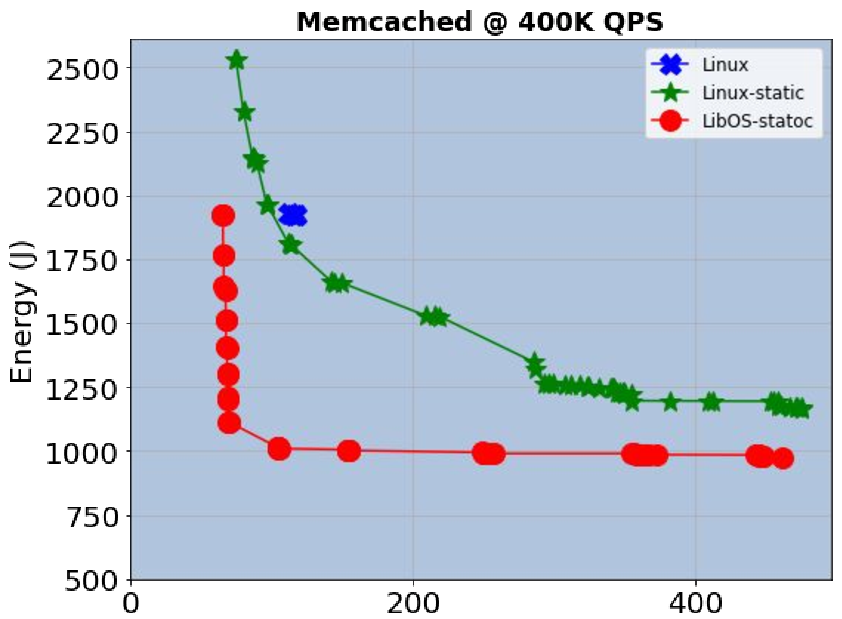
\includegraphics[width=1\textwidth]{img/mcd400K.pdf}
        \end{figure}
    \end{column}
    \begin{column}{.4\textwidth}
        \begin{itemize}
            \item Exploiting sleep states with ITR
            \item DVFS sensitivity to efficiency of OS
        \end{itemize}
    \end{column}
\end{columns}  
\end{frame}
%%%%%%%%%%%%%%%%%%%%%%%%%%%%

\begin{frame}{Rest of results for USENIX ATC}
\begin{columns}
    \begin{column}{.6\textwidth}
        \begin{figure}
            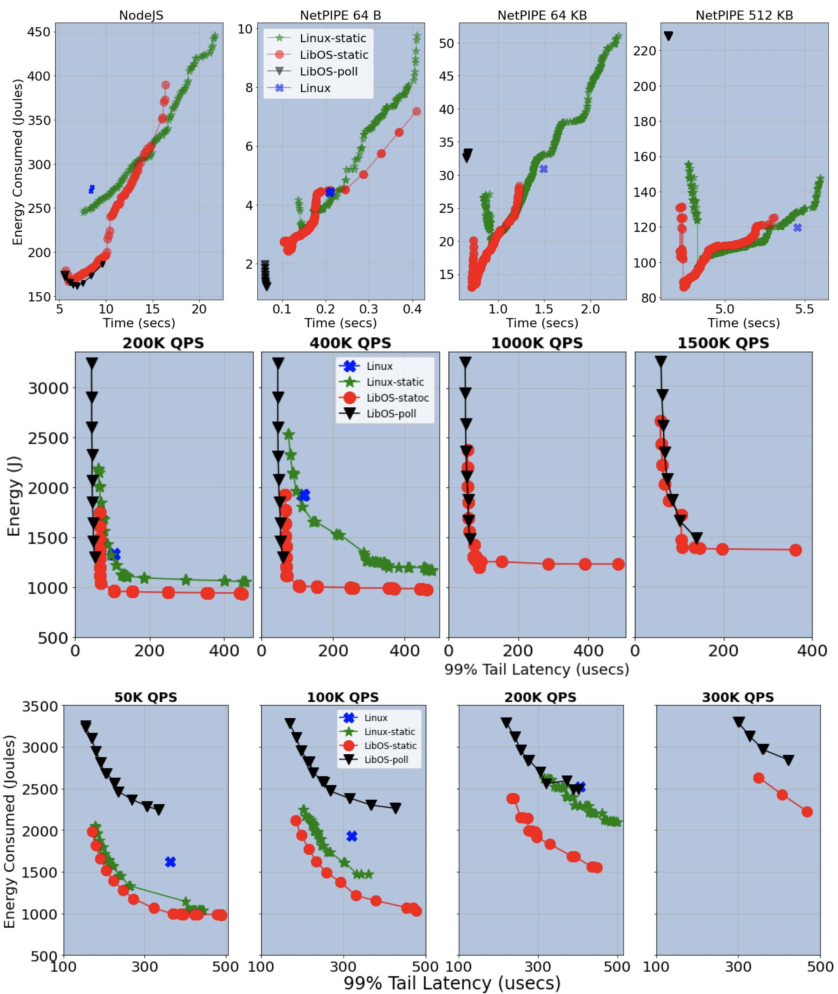
\includegraphics[width=1\textwidth]{img/atc_collage.pdf}
        \end{figure}
    \end{column}
    \begin{column}{.4\textwidth}
        \begin{itemize}
            \item Always an optimal static ITR, DVFS than default algorithms
            \item Specializing OS magnify both performance and energy
            \item Use insights from Linux results to explore new points in OS specialize space - polling
        \end{itemize}
    \end{column}
\end{columns}  
\end{frame}

% Exploiting OS specialization to do guided by data driven results to explore new points in this space
% As an example, we use polling


% Conclusion and Further work
\section{Conclusion and Further work}

\begin{frame}{Timetable}
\begin{table}[t]
\small
\begin{tabular}{l l}
(Proposed) Dates & Work To Be Done\\ \hline
completed & NIC driver analysis and port to EbbRT \\
completed & Get all applications to run on EbbRT, Linux \\
completed & Calibrate rack level energy consumption \\
completed & Build data collection infrastructure \\
completed & Collect data \\
completed & Fine-grained data analysis in EbbRT, Linux \\ 
completed & Static hardware settings results for performance/energy results \\ & - two papers under submission to ATC \\
Feb-Mar, 2022 & Apply data with modeling \\ & techniques and demonstrate \\ & prediction benefits (sigmetrics target) \\
Mar-April, 2022 & Draft of Completed Thesis to Committee \\
April-May, 2022 & Defense Date \\
Post Thesis, 2022 & Prototyping analysis of ML controller
\end{tabular}
\caption{Timeline for completion of the dissertation}
\label{table:timeline_thesis}
\end{table}
\end{frame}
%% Separate modeling from ML
%% Venn diagrams with 3 categories 

% Typically asked - time line for the project


% A thank you slide
\begin{frame}{\Large Thank you for your attention!}
  \centering \Large Any questions?
\end{frame}

\printbibliography

%\begin{frame}
%    \printbibliography
%\end{frame} 
 
\end{document}
